% Theme: Ritsumeikan University Theme Beamer Template
% https://www.overleaf.com/latex/templates/ritsumeikan-university-theme-beamer-template/jmfcqqptxjxk

\documentclass{beamer}
\usepackage{hyperref}
\usepackage[T1]{fontenc}

% other packages
\usepackage{latexsym,amsmath,xcolor,multicol,booktabs,calligra}
\usepackage{graphicx,pstricks,listings,stackengine}
\usepackage{ragged2e}

\author{Vishnu Sanal T}
\title{Software and Hardware Security of IoT}
\subtitle{CSQ413 SEMINAR}
\institute{
    Department of Computer Science \& Engineering \\
    Government Engineering College Palakkad
}
\date{October, 2023}

\usepackage{Ritsumeikan}

% defs
\def\cmd#1{\texttt{\color{red}\footnotesize $\backslash$#1}}
\def\env#1{\texttt{\color{blue}\footnotesize #1}}
\definecolor{deepblue}{rgb}{0,0,0.5}
\definecolor{deepred}{rgb}{0.6,0,0}
\definecolor{deepgreen}{rgb}{0,0.5,0}
\definecolor{halfgray}{gray}{0.55}

\lstset{
    basicstyle=\ttfamily\small,
    keywordstyle=\bfseries\color{deepblue},
    emphstyle=\ttfamily\color{deepred},    % Custom highlighting style
    stringstyle=\color{deepgreen},
    numbers=left,
    numberstyle=\small\color{halfgray},
    rulesepcolor=\color{red!20!green!20!blue!20},
    frame=shadowbox,
}


\begin{document}

\begin{frame}
    \titlepage
    \begin{figure}[htpb]
        \begin{center}
            
\includegraphics[keepaspectratio, scale=0.35]{pic/college_logo.png}
        \end{center}
    \end{figure}
\end{frame}

\begin{frame}
    \tableofcontents[sectionstyle=show,subsectionstyle=show/shaded/hide,subsubsectionstyle=show/shaded/hide]
\end{frame}

\section{Introduction}

\begin{frame}{Introduction}
    \begin{itemize} % [<+-| alert@+>] % stepwise alerts
        \item {IoT refers to the rapidly growing network of connected objects or devices that are able to collect and exchange data using sensors. \cite{qu_cr_2017}}
        \item {It has been proposed as an integral part of connected living. Thus in the next decade, IoT will have ubiquitous presence in the inhabited areas \cite{qu_cr_dev_2014}}
        \item {Security of IoT refers to the ways in which security is enforced in the IoT ecosystem.}
    \end{itemize}
\end{frame}

\section{Motivation}

\begin{frame}{Motivation}
    \begin{itemize}
        \item {The extent of exposure of us, human beings, to devices that are connected to the internet in our day-to-day life.}
        \item {This in itself brings in lots of security risks \& privacy concerns, which we'll discuss shortly.}
        \item {This seminar sheds light on the ways in which security can be enforced on IoT devices on software \& hardware levels.}
    \end{itemize}
\end{frame}

\section{Objectives}

\begin{frame}{Objectives}
    \begin{itemize}
        \item {To understand Security Concerns of IoT}
        \item {To analyse techniques to enhance the Security of IoT devices in the hardware \& software levels}
    
    \end{itemize}
\end{frame}

\section{Abstract}

\begin{frame}{Abstract}
    \begin{itemize}
        \item {With the monumental advent of IoT devices in our day to day life, providing security to them has risen to be a critical issue.}
        \item {This seminar aims to shed light into techniques that can be used to ensure the safety of Internet of Things (IoT) devices.}
        \item {Security techniques include techniques that make use of hardware specifications \& techniques that are enforced in the software level.}
    \end{itemize}
\end{frame}

\section{Problem Definition}

\begin{frame}{Security Concerns of IoT}
    \begin{itemize}
        \item {IoT devices deal with sensitive information (health conditions, whereabouts, etc) which makes it more prone to eavesdropping \cite{qu_cr_2017}}
        \item {Complex management of mass amount of sensor nodes, heterogeneity, and lack of agreed standards, makes an easy target. \cite{qu_iot_2019}}
        \item {Hardware trojans i.e, unwanted circuits which are leaking the data. \cite{sw_hw_sec_2021}}        
    \end{itemize}
\end{frame}

\begin{frame}{Security Concerns of IoT: Security problems on each layer}
    \begin{itemize}
        \item {Perception Layer: The attackers add a node to the system, and input fake code or data. \cite{su_iot_2013}}
        \item {Network Layer: A large number of malicious nodes send data at the same time; a DoS attack. \cite{su_iot_2013}}
        \item {Application Layer: Illegal user intervention, identification \& processing of spam and malicious information. \cite{su_iot_2013}}
    \end{itemize}
\end{frame}

\begin{frame} {Techniques to enhance the security of IoT devices}

    \justifying {We have to provide security at every level, i.e, from hardware level to the software level. \cite{sw_hw_sec_2021}}

    \begin{itemize}
    
    \item {Hardware Level Security}
        \begin{itemize}
            \item {Integrating specialised logic circuits}
        \end{itemize}
        \item {Software Level Security (Data Transmission Level)}
        \begin{itemize}
            \item {Use Blockchain technology in order to have secure peer to peer communication}
            \item {Integrating Quantum cryptography to make sure that the data on the network is safely encrypted}
        \end{itemize}
        
    \end{itemize}
\end{frame}

\begin{frame}{Hardware Security}
    \begin{itemize}
        \item {Installing or fabricating a fake or dummy logic.}
        \item {Implementing multiple modes of operation like normal mode and malfunction node.}
        \item {Installing a built-in self-test circuit.}
    \end{itemize}
\end{frame}

\begin{frame}{Software Security: Blockchain Technology}
    \justifying {What is Blockchain?}
    \begin{itemize}
        \item {Blockchain, also known as Distributed Ledger Technology, is designed to support verification-driven transaction services within a generally untrusted ecosystem. \cite{art_ch_2019}}
        \item {This design ensures that no one entity can modify a record in the ledger without consensus from other network participants. \cite{art_ch_2019}}
        \item {This ensures the immutability of data stored on the ledger. \cite{art_ch_2019}}
    \end{itemize}
\end{frame}

\begin{frame}{Components of Blockchain \cite{sw_hw_sec_2021}}

\begin{minipage}{0.5\textwidth}
        \begin{figure}
           \centering
           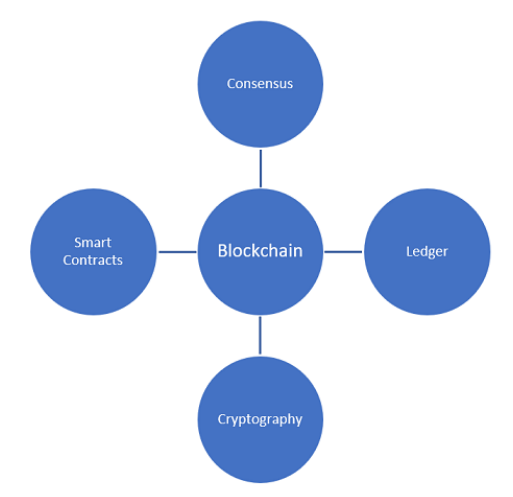
\includegraphics[width=0.75\linewidth]{pic/blockchain_components.png}
           \caption{Components of Blockchain}
          \label{fig:components-of-blockchain}
      \end{figure}
\end{minipage}%
\begin{minipage}{0.5\textwidth}
    \centering
    \begin{itemize}
        \item {Ledger: Provides the details of the transactions that occurred between the nodes.}
        \item {Smart Contract:  Programs that run when predetermined conditions are met. Used for verification and validation of the connecting nodes.}
    \end{itemize}
\end{minipage}
\end{frame}

\begin{frame}{Components of Blockchain \cite{sw_hw_sec_2021}}

\begin{minipage}{0.5\textwidth}
        \begin{figure}
           \centering
           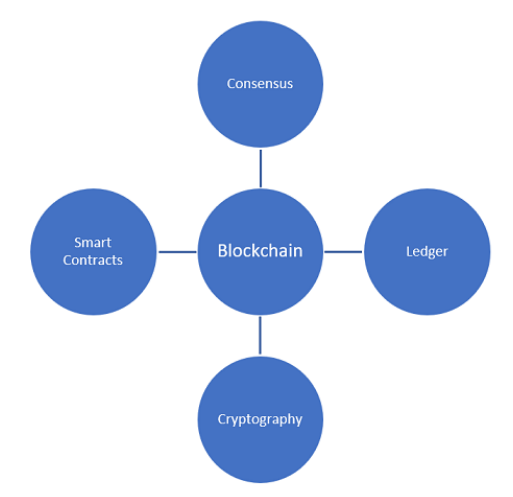
\includegraphics[width=0.75\linewidth]{pic/blockchain_components.png}
           \caption{Components of Blockchain}
          \label{fig:components-of-blockchain-2}
      \end{figure}
\end{minipage}%
\begin{minipage}{0.5\textwidth}
    \centering
    \begin{itemize}
        \item {Consensus: Proof of work that verifies the actions occurring around the networks.}
        \item {Cryptography: The data is secured using cryptographic techniques and unauthorised users cannot alter the data.}
    \end{itemize}
\end{minipage}
\end{frame}

\begin{frame}{Architecture of IoT based on Blockchain \cite{sw_hw_sec_2021}}

\begin{minipage}{0.5\textwidth}
        \begin{figure}
            \centering
            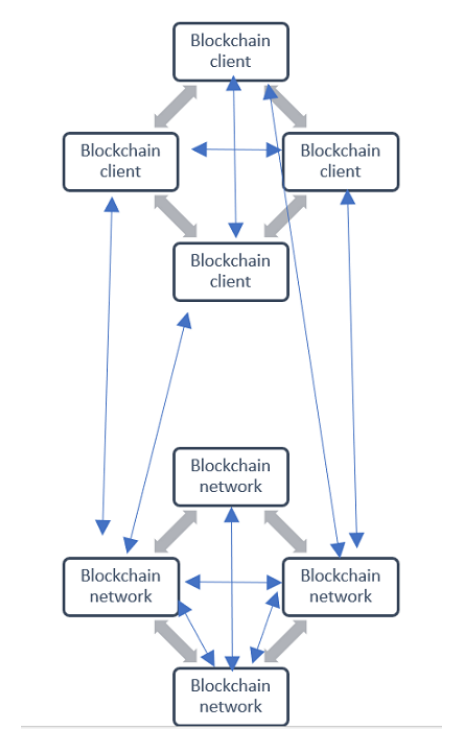
\includegraphics[width=0.7\linewidth]{pic/distributed_data_sharing.png}
            \caption{Distributed Data Sharing}
            \label{fig:distributed-data-sharing}
        \end{figure}
\end{minipage}%
\begin{minipage}{0.5\textwidth}
    \centering
    \begin{itemize}
        \item {Each IoT node is the member of the network participating in the transaction.}
        \item {These IoT devices are the client and these clients will interact with each other with APIs.}
    \end{itemize}
\end{minipage}
\end{frame}

\begin{frame}{Architecture of IoT based on Blockchain \cite{sw_hw_sec_2021}}

\begin{minipage}{0.5\textwidth}
        \begin{figure}
            \centering
            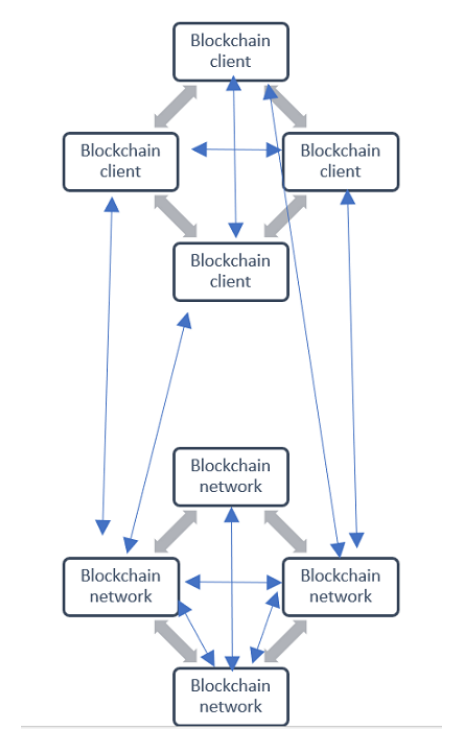
\includegraphics[width=0.7\linewidth]{pic/distributed_data_sharing.png}
            \caption{Distributed Data Sharing}
            \label{fig:distributed-data-sharing-2}
        \end{figure}
\end{minipage}%
\begin{minipage}{0.5\textwidth}
    \centering
    \begin{itemize}
        \item {Devices create transactions and these transactions are sent to the blockchain nodes for storing and processing data into distributed ledger.}
        \item {REST APIs can be used to make communication with the IoT devices and the blockchain.}
    \end{itemize}
\end{minipage}
\end{frame}

\begin{frame}{Software Security: Quantum Cryptography \cite{qu_cr_2017}}
    \begin{itemize}
        \item {What is Cryptography?}
        \item {QC is based on the fundamental and consistent principles of quantum mechanics.}
        \item {QC does not transmit any message signal, instead only used to produce and distribute a key.}
        \item {BB84 Protocol is the earliest and one of the most famous Quantum key distribution protocols.}
    \end{itemize}
\end{frame}

\begin{frame}{Software Security: Quantum Cryptography \cite{qu_cr_2017}}

\begin{minipage}{0.4\textwidth}
    \begin{table}
        \centering
        \begin{tabular}{|c|}
        \hline
            Application Layer\\
        \hline
            Quantum Security Layer\\
        \hline
            Network Layer\\
        \hline
            Perception layer\\
        \hline
        \end{tabular}
        \caption{IoT Layers}
        \label{tab:iot_layers}
    \end{table}
\end{minipage}%
\begin{minipage}{0.6\textwidth}
    \begin{itemize}
        \item {There are 3 layers (perception layer, network layer, application layer) in a classical IoT system.}
        \item {The proposed system has an additional layer “Quantum Security Layer” (introduced before application layer) which only protects the security key.}
        \item {The other layers communicate in between using the same classical approach.}
    \end{itemize}
\end{minipage}
\end{frame}

% At first Alice will send some qubits containing a random key.

% Bob will measure this qubits in random choices of bases. It can be general basis, or sign basis or any orthonormal basis.

% Then Bob calls Alice, confirm his completion of measurement.

% Alice then tells Bob the correct basis to measure the qubit. In that case, Bob will surely know which measurement result is the key to encode the information passing through the classical communication channel.

\begin{frame}{Software Security: Adapted BB84 Protocol \cite{qu_iot_2019}}
    \begin{enumerate}
        \item {Start}
        \item {Alice generated a random bit string d}
        \item {Alice send ‘start’ signal}
        \item {Bob send ‘ACK’ signal}
        \item {Alice send qubit data}
    \end{enumerate}
\end{frame}

\begin{frame}{Software Security: Adapted BB84 Protocol \cite{qu_iot_2019}}
    \begin{enumerate}
        \setcounter{enumi}{6}
        \item {For d = 0 bit, qubit state is general (|0 and |1)}
        \item {For d = 1 bit, qubit state is sign (|+ and |-)}
        \item {Bob measure qubit in both sign and general basis}
        \item {Alice using one time pad let bob know the exact basis}
        \item {Bob choose the value regarding basis [general basis: d = 0; sign basis: d = 1;)}
    \end{enumerate}
\end{frame}

\begin{frame}{Software Security: Adapted BB84 Protocol \cite{qu_iot_2019}}
    \begin{enumerate}
    \setcounter{enumi}{11}
        \item {Alice send ‘stop’ signal}
        \item {Bob send ‘ACK’ signal}
        \item {Bob perform classical coding method to finally retract the information}
        \item {Stop}
    \end{enumerate}
\end{frame}

% \section{Literature Survey}

% \begin{frame}{{Literature Survey \textit{todo:}}}
%     \justifying {\textit{todo: what here?}}
% \end{frame}

\section{Conclusion}

\begin{frame}{Conclusion}
    \begin{itemize}
        \item {Discussed about the Security Concerns of IoT devices}
        \item {Performed analysis of techniques to enhance the Security of IoT devices in the hardware \& software levels}
    \end{itemize}
\end{frame}

\section{References}

\begin{frame}[allowframebreaks]
    \bibliography{ref}
    \bibliographystyle{ieeetr}
    % \nocite{*} % used here because no citation happens in slides
    % if there are too many try use:
    % \tiny\bibliographystyle{alpha}
\end{frame}

\begin{frame}
    \begin{center}
        {\Huge\calligra You're Awesome :)}
    \end{center}
\end{frame}

\end{document}